\documentclass[reqno,12pt,oneside]{report}\usepackage[]{graphicx}\usepackage[]{color}
%% maxwidth is the original width if it is less than linewidth
%% otherwise use linewidth (to make sure the graphics do not exceed the margin)
\makeatletter
\def\maxwidth{ %
  \ifdim\Gin@nat@width>\linewidth
    \linewidth
  \else
    \Gin@nat@width
  \fi
}
\makeatother

\definecolor{fgcolor}{rgb}{0.345, 0.345, 0.345}
\newcommand{\hlnum}[1]{\textcolor[rgb]{0.686,0.059,0.569}{#1}}%
\newcommand{\hlstr}[1]{\textcolor[rgb]{0.192,0.494,0.8}{#1}}%
\newcommand{\hlcom}[1]{\textcolor[rgb]{0.678,0.584,0.686}{\textit{#1}}}%
\newcommand{\hlopt}[1]{\textcolor[rgb]{0,0,0}{#1}}%
\newcommand{\hlstd}[1]{\textcolor[rgb]{0.345,0.345,0.345}{#1}}%
\newcommand{\hlkwa}[1]{\textcolor[rgb]{0.161,0.373,0.58}{\textbf{#1}}}%
\newcommand{\hlkwb}[1]{\textcolor[rgb]{0.69,0.353,0.396}{#1}}%
\newcommand{\hlkwc}[1]{\textcolor[rgb]{0.333,0.667,0.333}{#1}}%
\newcommand{\hlkwd}[1]{\textcolor[rgb]{0.737,0.353,0.396}{\textbf{#1}}}%
\let\hlipl\hlkwb

\usepackage{framed}
\makeatletter
\newenvironment{kframe}{%
 \def\at@end@of@kframe{}%
 \ifinner\ifhmode%
  \def\at@end@of@kframe{\end{minipage}}%
  \begin{minipage}{\columnwidth}%
 \fi\fi%
 \def\FrameCommand##1{\hskip\@totalleftmargin \hskip-\fboxsep
 \colorbox{shadecolor}{##1}\hskip-\fboxsep
     % There is no \\@totalrightmargin, so:
     \hskip-\linewidth \hskip-\@totalleftmargin \hskip\columnwidth}%
 \MakeFramed {\advance\hsize-\width
   \@totalleftmargin\z@ \linewidth\hsize
   \@setminipage}}%
 {\par\unskip\endMakeFramed%
 \at@end@of@kframe}
\makeatother

\definecolor{shadecolor}{rgb}{.97, .97, .97}
\definecolor{messagecolor}{rgb}{0, 0, 0}
\definecolor{warningcolor}{rgb}{1, 0, 1}
\definecolor{errorcolor}{rgb}{1, 0, 0}
\newenvironment{knitrout}{}{} % an empty environment to be redefined in TeX

\usepackage{alltt} % right-side equation numbering, 12 point font, print one-sided 

\usepackage{etoolbox}
\newtoggle{draft}
\toggletrue{draft}
\togglefalse{draft}


\usepackage{amsmath}
\usepackage{rac}         % Use Rackham thesis style file
\usepackage{acronym}
\usepackage{amsxtra}     % Use various AMS packages
\usepackage{amsthm}
\usepackage{amssymb}
\usepackage{amsfonts}
\usepackage{graphicx}    % Add some packages for figures. Read epslatex.pdf on ctan.tug.org
\usepackage{color}
\usepackage{subfigure}   % To make subfigures. Read subfigure.pdf on ctan.tug.org
\usepackage{verbatim}

\usepackage{hyperref}

%\setlength\fboxsep{5cm}

\ifdefined\knitrout
  \renewenvironment{knitrout}{\begin{small}}{\end{small}}
\else
\fi

\usepackage{xcolor}
\hypersetup{
    colorlinks,
    linkcolor={black!50!black},
    citecolor={blue!50!black},
    urlcolor={blue!80!black}
}

\usepackage{courier}
\usepackage{listings}
\lstset{
numbers=left, 
numberstyle=\small, 
numbersep=8pt, 
frame = single, 
language=Pascal, 
framexleftmargin=25pt,
breaklines=true,
basicstyle=\footnotesize\ttfamily,
commentstyle=\textsl,
keywordstyle=\mdseries,
showstringspaces=false,
index=[1][keywords]}

\usepackage{nicefrac}
\usepackage{stmaryrd}
\usepackage{lipsum}
\usepackage[inline]{enumitem}

\usepackage{natbib}      % Allows you to use BibTeX
\bibliographystyle{abbrvnat}
\setcitestyle{authoryear}

\usepackage{setspace}    % Allows you to specify the line spacing
\doublespacing           % \onehalfspacing for 1.5 spacing, \doublespacing for 2.0 spacing.

\iftoggle{draft}{
  \usepackage[paperheight=13in,paperwidth=13in,  % or: "paper=a4paper"
    layoutheight =11in,layoutwidth=8.5in,
    layoutvoffset= 1in,layouthoffset=.5in,
    left = .5in,
    right =.5in,
    top =.5in,
    bottom =.5in,
    showframe=false, showcrop=true]{geometry}
  \setlength{\marginparwidth}{4in}
  \usepackage[colorinlistoftodos,color=pink,textsize=singlespacetiny]{todonotes}
  \newcommand{\singlespacetiny}{\linespread{1}\normalsize}
  \usepackage[pagewise]{lineno}
  \linenumbers
  \setlength\linenumbersep{30pt}
  \renewcommand\thelinenumber{{\normalsize {\color{lightgray}{\bf\arabic{linenumber}}}}}
}{
  \usepackage[colorinlistoftodos,color=white]{todonotes}
    \usepackage[paper=letterpaper,
    left = .5in,
    right =.5in,
    top =.5in,
    bottom =1in]{geometry}

    \renewcommand{\todo}[2][]{}
}

\renewcommand{\citet}[1]{(\citeauthor{#1} \citeyear{#1})}




%%%%%%%%%%%%%%%%%%%%%%%%%%%%%%%%%%%%%%%%%%%%%%%%%%%%%%%%%%%%%%%%%%%%%%%%%%%%%%%

% Various theorem environments. All of the following have the same numbering
% system as theorem.

\theoremstyle{plain}
\newtheorem{theorem}{Theorem}
\newtheorem{prop}[theorem]{Proposition}
\newtheorem{corollary}[theorem]{Corollary}
\newtheorem{lemma}[theorem]{Lemma}
\newtheorem{question}[theorem]{Question}
\newtheorem{conjecture}[theorem]{Conjecture}
\newtheorem{assumption}[theorem]{Assumption}

\theoremstyle{definition}
\newtheorem{definition}[theorem]{Definition}
\newtheorem{notation}[theorem]{Notation}
\newtheorem{condition}[theorem]{Condition}
\newtheorem{example}[theorem]{Example}
\newtheorem{introduction}[theorem]{Introduction}

\theoremstyle{remark}
\newtheorem{remark}[theorem]{Remark}
%%%%%%%%%%%%%%%%%%%%%%%%%%%%%%%%%%%%%%%%%%%%%%%%%%%%%%%%%%%%%%%%%%%%%%%%%%%%%%%

\numberwithin{theorem}{chapter}     % Numbers theorems "x.y" where x
                                    % is the section number, y is the
                                    % theorem number

%%%%%%%%%%%%%%%%%%%%%%%%%%%%%%%%%%%%%%%%%%%%%%%%%%%%%%%%%%%%%%%%%%%%%%%%%%%%%%

% If printing two-sided, this makes sure that any blank page at the 
% end of a chapter will not have a page number. 
\makeatletter
\def\cleardoublepage{\clearpage\if@twoside \ifodd\c@page\else
\hbox{}
\thispagestyle{empty}
\newpage
\if@twocolumn\hbox{}\newpage\fi\fi\fi}
\makeatother 

%%%%%%%%%%%%%%%%%%%%%%%%%%%%%%%%%%%%%%%%%%%%%%%%%%%%%%%%%%%%%%%%%%%%%%%%%%%%%%

%This command creates a box marked ``To Do'' around text.
%To use type \todo{  insert text here  }.

%\newcommand{\todo}[1]{\vspace{5 mm}\par \noindent
%\marginpar{\textsc{To Do}}
%\framebox{\begin{minipage}[c]{0.95 \textwidth}
%\tt\begin{center} #1 \end{center}\end{minipage}}\vspace{5 mm}\par}

%%%%%%%%%%%%%%%%%%%%%%%%%%%%%%%%%%%%%%%%%%%%%%%%%%%%%%%%%%%%%%%%%%%%%%%%%%%%%%%
\IfFileExists{upquote.sty}{\usepackage{upquote}}{}
\begin{document}

\newcommand{\mytitle}{A New Approach to Sample Deconvolution}

% Title page as required by Rackham dissertation guidelines
\titlepage{\mytitle}{Gregory Hunt}{Doctor of Philosophy}
{Statistics}{2016}
{Assistant Professor Johann Gagnon-Bartsch, Chair\\
Professor Kerby Shedden\\
 Professor Naisyin Wang}

% Begin the front matter as required by Rackham dissertation guidelines
\initializefrontsections

% Page numbering. If you don't include a frontispiece or copyright page, you'll need to change this for two-sided printing.
\makeatletter
\if@twoside \setcounter{page}{4} \else \setcounter{page}{1} \fi
\makeatother

% Optional Preface page
%\startprefacepage
%\input{Preface}
%\label{Preface}

% Table of contents, list of figures, etc.
\tableofcontents     % Required
%\listoffigures       % Required if there is more than one figure
%\listoftables        % Required if there is more than one table
%\listofmaps          % Required if there is more than one map
%\listofappendices    % Required if there is more than one appendix
%\listofabbreviations % Optional. Abbreviations should be stored in a file named abbr.tex

% Optional in-dissertation Abstract Page
\startabstractpage{\mytitle}{Greg Hunt}{}

\lipsum[1]
\label{Abstract}

\startthechapters 
% The individual files for each of the chapters are put here.
% Save each chapter of your thesis to a seperate tex file
% and then use the \input command to include this file in your
% thesis.  For instance you can save a file to "intro.tex" and 
% then type \input{intro}. 

 \chapter{Introduction}
 \label{chap:Intro}

High-throughput gene expression profiling technologies such as DNA microarrays and RNA sequencing have become important microbiological tools. Their power and popularity come from their ability to make a large number of simultaneous measurements. Such technologies allow the measurement of tens of thousands of gene expressions. This gives biologists a high-level view of genome activity as well as allowing investigation of individual genes. While these profiling techniques have proven to be invaluable tools their analyses are not without caveats. One issue which confounds gene expression profiling is sample heterogeneity. 

Profiling techniques measure gene expression of a sample. A sample is simply a collection of cells. These cells typically are cultivated from animal tissue, for example, a rat tumor biopsy or human blood titer. The gene expressions measured reflect the average gene expression across cells in the sample. Thus, for a sample consisting of precisely one cell type the measurements typify a gene expression profile for that type. However, for a heterogeneous sample of several cell types the measured expressions are not as interpretable. In this case the measurements will be a convolution of the expression profiles from the constituent types. 

The convoluted nature of heterogeneous data makes comparing expression measurements across samples difficult. It becomes necessary to determine if changes in measurements come from genuine expression changes in cells or from compositional changes affecting the samples' mixing proportions. More to the point, it is often of interest to analyze expression changes in individual cell types and not a mixture thereof. Unfortunately heterogeneous samples are the rule not the exception and comparative analyses, like differential expression analysis, are a primary application of interest.

Accordingly, researchers have two goals when dealing with heterogeneous data. First, they would like to remove any confounding effects of sample heterogeneity. Secondly, they want to be able to get cell subtype specific gene expression profiles. Methods to these ends are dubbed \emph{cell type deconvolution}. Solutions have been pioneered at both the physical cell sample level and data analytic level. Physical techniques like flow cytometry attempt to solve the heterogeneity problems by sorting cells into their respective types before analysis is performed. These techniques are employed to purify heterogeneous samples into homogeneous ones allowing researchers to be sure that the final samples analyzed contain only one cell type. However these techniques are expensive, time intensive and have been noted to change gene expression. Thus, in lieu of physical methods, there is ample room for data analytical techniques to deconvolve expression signal from heterogeneous samples. 

 

 \chapter{Scientific Background}
 \label{chap:Science}

All gene profiling techniques involve the so-called \emph{central dogma of genetics}. That is, DNA is transcribed into messenger RNA (mRNA) and mRNA is translated into proteins. Thus, to a first approximation, when looking to determine which genes are being expressed by a cell one needs only look at what mRNA is being created by a cell. This follows because every time a gene is expressed an mRNA molecule specific to that gene is produced.

This one-to-one correspondence between gene expression and mRNA production is exploited by gene profiling techniques. A profiling experiment starts with a sample of cells. From these cells the mRNA is extracted and quantified. The scientist then fragments some fixed amount of this mRNA for use in analysis. Fragmentation is the process of breaking up long mRNA molecules into smaller chunks. This aids in the main profiling pursuit, namely, identification of the mRNA. The goal is to determine which species of mRNA is present. Determining what types of mRNA is present will tell scientists which genes are being expressed. Each of the many profiling techniques have a different way of determining what types of mRNA is present. For example, RNA-Seq determines the base-pair ordering on the mRNA fragments. These base-pair sequences can then be mapped to mRNA molecules and subsequently genes. On the other hand, DNA microarrays determine mRNA quantities by fluorescent tagging. Our discussion in this paper will focus mainly on DNA microarray technology.

A DNA microarray is a small chip (about one inch on a side) resembling a microscope slide. The surface of the chip is divided up into an array of squares we will call ``probe squares.'' Each of these probe squares will probe for mRNA fragments containing a specific base sequence. That is, each of the squares will be used to measure the amount of a specific type of mRNA fragment. Hence we can map each of these squares from the fragment type they measure to a specific mRNA molecule and thus a specific gene. In this way we can determine the expression of a gene in our sample. We do this by looking at all the probes sensitive to mRNA fragments produced by the gene. The probe squares will tell us about gene expression as follows. To each of the probe squares on the microarray there are affixed thousands of nucleic acid fragments called probes. Each of the probes on a probe square have base-pair sequences complementary to one specific mRNA fragment type. Thus the probes on any particular probe square will hybridize to one specific species of mRNA fragment. The scientist then fluorescently tags the mRNA fragments extracted from the cell sample. These fluorescently tagged mRNA fragments are then put on the DNA microarray. The tagged fragments will hybridize to their complementary probes which are located on a specific probe square. All non-hybridized fragments are washed from the microarray. The array is then hit with a laser to excite the hybridized and fluorescently tagged sample fragments. If a gene is being expressed highly in the cell sample then there will be a lot of its mRNA molecules present and thus many fluorescently tagged mRNA fragments corresponding to that gene. Once hybridized to the array and hit with a laser the probe squares sensitive to mRNA fragments from that gene will fluoresce brightly. They fluoresce brightly because there are many fluorescently tagged mRNA  fragments hybridized to their probes. Thus we see that the gene is highly expressed because its probe squares are fluorescing a lot. On the other hand if a gene is not being expressed much by cells in our sample there will be relatively few of its mRNA molecules and subsequently few of its fluorescently tagged fragments. Thus the probe squares corresponding to this gene will fluoresce only a little as there are not many tagged fragments available to hybridize to the probes. In this way we can look at the microarray and determine which genes are relatively highly expressed by looking at which probe squares are lighting up brightly. To enable quantitative analysis of the microarray a picture is taken of the fluorescing array. For each of the probe squares in the picture a fluorescence intensity is recorded. Thus for each probe square on the microarray the scientists get an intensity measurement that is positively related to the expression of a particular gene in our sample. We call these measurements the probe-level intensity measurements. In many cases these probe-level measurements are summarized to a gene-level by aggregating all the probe intensities related to a particular gene. 

In any case, whether we are working with DNA microarrays or RNA-seq or some other profiling technology the data analyst gets a list of genes and corresponding expression signals. Sometimes (as when working with probe-level data) there are repeated measurements such that each gene has several measurements somehow capturing its expression. Furthermore there are often pre-processing and post-processing adjustments and transformations applied to gene expressions. Regardless, the expression signals a scientist gets through one of these methods are positively related to the average expression of a gene by the cells in the sample. 

 \chapter{Literature Review}
 \label{chap:Lit}

The first computational method for cell type deconvolution is generally attributed to \cite{Venet2001}. Since then there has been much activity in this area with dozens of methods published as recently as this past year \citet{Newman2015}. Notably, the model used for cell type deconvolution is largely the same across methods. Authors use some version of a linear model. There are, however, important differences in data assumptions and fitting methods to be considered. Our attempt here is to lay out a comprehensive, yet concise, survey of existing cell type deconvolution methodology.

\section{Model Basics}

Let's assume that for any cell sample we make $N$ expression measurements. We are purposely ambiguous here about exactly what we mean by `` expression measurements.'' For a DNA microarray these $N$ measurements may be probe-level intensity measurements. They may also be gene-level expressions summarizing the probe intensities by an algorithm like MAS5 \citet{Hubbell2002} or RMA \citet{Irizarry2003}. Furthermore, while we focus on DNA microarrays, the methods presented are likely easily applicable to some transformed mRNA counts from RNA-seq. In any case each of the $N$ measurements captures the quantity of some nucleic acid in our sample. For ease of terminology we will henceforth refer to the nucleic acid fragments measured by each of the $N$ expressions as ``oligonucleotides'' or, concisely, ``oligos.'' Depending on context the measurement of a ``oligo'' may refer to the expression measurement of some mRNA fragment itself or to the summary measurement of all the mRNA transcripts from a gene. Without loss of generality we can label these oligos from $1$ to $N$. We will need to assume that some of these oligo measurements are ``characteristic'' of a particular cell type. We call these ``characteristic oligos.'' An oligo is characteristic of a particular cell type if it is abundant in cells of that type and not abundant in cells of any other type. The hope is that these characteristic oligos will allow us to distinguish among cell types. 

Usually experiments are done in batches. Let's assume that we have $S$ cell samples and conduct the same assay on each of the samples. Let $X_{sn}$ be the expression measurement of the $n^{th}$ oligo in the $s^{th}$ sample. Then the matrix $X\in \mathbb{R}^{S \times N}$ has rows $X_{s}$ each containing the expression measurement of all $N$ oligos in sample $s$. The columns of $X$, denoted $X^n$, are the expression measurements of the $n^{th}$ oligo across all samples. Furthermore posit that each of the $s$ samples is a heterogeneous mixture of $K$ cell types. Define the mixing matrix $M \in \mathbb{R}^{S \times K}$ to be so that $M_{sk}$ is the percent of sample $s$ comprised of cells of type $k$. The rows of $M$ are the mixing proportions of the $K$ cell types in the $s^{th}$ sample meaning that $M$ is row-wise a probability matrix. Finally define the matrix $U \in \mathbb{R}^{K \times N}$ to be the matrix of characteristic oligo measurements. Specifically $U_{kn}$ is the typical oligo expression of oligo $n$ in cell type $k$. Each row of the matrix, $U_{k}\in\mathbb{R}^{N}$, is what we call a oligo expression profile for type $k$. It is a vector that contains the ``characteristic'' or ``typical'' expression measurements of cells of type $k$ for each of the $N$ oligos.

By and far the most common manner to model cell-type convolution is as a linear model such that
\begin{equation}
  \label{mainmodeqn}
X = MU + E
\end{equation}
where $E$ is a random matrix of errors. Almost universally cell-type convolution is modeled as such a matrix product of $M$ and $U$ however most of the deconvolution literature does not explicitly state such a statistical model. Mainly authors do not discuss an error term $E$ much less its distribution. Thus we are correspondingly vague about $E$. 

This model is attractive because it is simple. The model posits that the convoluted expressions from heterogeneous mixtures of $K$ cell types, as captured in $X$, are linear combinations of some ``characteristic'' expressions of each of the $K$ types, captured by $U$, with weights that are simply the mixing proportions of the types in each of the samples, the matrix $M$. Put another way, cell type convolution is a linear mixing process. Some version of this linear mixing model is used in all the methods we surveyed. While the true relation between the characteristic expression profiles $U$ and the convoluted data $X$ is known to be non-linear this model has proven both approximately true and empirically quite useful \citet{Shen-Orr2010}.

Beyond this basic model there are several facets which set apart existing deconvolution techniques. Firstly there are the assumptions about which data is known. As $X$ is the data we want to deconvolve, it is always assumed that $X$ is known. However we can posit either knowing $M$ to predict $U$ or knowing $U$ to predict $M$ or knowing neither $M$ nor $U$ and jointly estimating them. Hand in hand with these data assumptions are the preprocessing normalizations and transformations applied to the data by the authors. The second major facet to a deconvolution algorithm is the marker oligos. Marker oligos are expression measurements that are particularly indicative of one cell type over the others. It has been noted almost universally that restricting analysis to these marker oligos, in one way or another, can improve model fit. Thus the manner in which the markers are chosen and applied set apart the deconvolution techniques. Finally, the approach to fitting the linear model distinguishes the methods. Part of the choice when fitting the model is what constraints to enforce. For example, we would like the mixing proportions to be positive and sum to one.

For this paper we are mostly interested in methods that can predict the mixing proportions $M$. Thus we begin by focusing on methods where $U$ is assumed to be known and $M$ is inferred. We will then talk about methods of estimating $U$ and $M$ jointly without prior knowledge or either. We will not discuss methods that assume the mixing proportions $M$ are known and attempt to predict $U$.  

\section{Known Characteristic Profiles}
\label{litrev:knownu}

Let's look at methods of cell type deconvolution where the expression profile matrix $U$ is known and one is interested in estimating the mixing matrix $M$. The simplest such algorithms comes from \cite{Abbas2009}. Here the authors work with linearly summarized gene level microarray data normalized by the  MAS5 algorithm. The cell type expression profiles are gathered either from external databases or created from expression profiles of known pure mixtures. The convolution problem is modeled as in equation \ref{mainmodeqn}. The mixing matrix $M$ is thus estimated by regressing the convoluted profiles $X$ on the known expression profiles $U$ using by a linear least squares optimization. The fit is done using only a subset of marker oligos (genes in this case) chosen by a combination of biological knowledge and differential expression of genes between the cell types as measured by absolute differences and t-test $p$-values of the gene expressions. The precise marker genes are then chosen by minimizing the condition number of the resulting sub-matrix of $U$. To enforce the sum-to-one (STO) and non-negativity (NN) constraints on the rows of the resulting estimate of $M$ a heuristic iterative algorithm is used which involves removing the smallest negative estimated regression coefficient and refitting the model. The rows of the estimated $M$ matrix are then re-scaled such that they sum to one. An implementation of their algorithm in \verb+R+ \citet{R2016} is available as part of the \verb+CellMix+ package \citet{Gaujoux2013}.

A similar approach to \citeauthor{Abbas2009} is taken by \cite{Gong2011} following the model in equation \ref{mainmodeqn}. However, in this paper \citeauthor{Gong2011} work with RMA summarized log-level gene expression data from microarrays as opposed to linearly summarized data. Marker genes are chosen in a similar fashion to \citeauthor{Abbas2009} but the model is fit using quadratic programming instead of regression. The quadratic programming framework allows explicit encoding of the NN and STO constraints. An implementation of this algorithm is also available as part of the \verb+CellMix+ package.

In a similar fashion the linear model in equation \ref{mainmodeqn} is used in \cite{Lu2003} and \cite{Wang2006} to estimate the mixing proportions $M$ using simulated annealing. \citeauthor{Lu2003} deconvolve log-level standardized microarray data using their algorithm \verb+DECONVOLUTE+ (no implementation currently available). Notably they do not use marker genes although they do mention that such genes may be useful for fitting. Meanwhile \cite{Wang2006} implement a similar algorithm at the linear gene level (normalized by MAS5) and choose to fit only using marker genes. Marker genes are found by differential expression analysis between pure cell type expression profiles using direct comparison, t-test $p$-values and step-wise discriminant analysis. No implementation of their algorithm is currently available.

Other ways to fit the linear model can be found in \cite{Qiao2012} who implement an algorithm using non-negative least squares. \cite{Qiao2012} work with log-level gene expression data normalized by RMA. The use of non-negative least squares allows them to deal with the NN constraint. The STO constraint is handled by post hoc re-normalizing the rows of the estimated $M$ matrix such that they sum to one. Marker genes are chosen by differential expression comparisons between pure expression profiles of the types. An implementation of their algorithm in \verb+Octave+ can be found in the supplemental material of their paper \citet{Qiao2012}. 

\cite{Newman2015} and \cite{Altboum2014} fit the linear model using penalized fitting methods. \citeauthor{Altboum2014} use an elastic-net penalization to deconvolve log-transformed RNA-seq data. They compare their method across several ways of choosing marker genes. Their algorithm, named \verb+DCQ+ for ``digital cell quantification'',  is available as part of the \verb+ComICS+ package in \verb+R+ \citet{ComICS2016}. On the other hand, \citeauthor{Newman2015} solve the model using support vector regression, specifically $\nu$-SVR with a linear kernel. They look at linear normalized gene-level data and, similar to others, choose marker genes looking at differential expressions across groups by $p$-values and the 2-norm condition number of the resulting cell type profile sub-matrices. The NN constraint is dealt with by zeroing out negatively estimated mixing proportions and the STO constraint is then satisfied by re-scaling the mixing proportions so they sum to one. Their algorithm, dubbed \verb+CIBERSORT+, is available in \verb+R+ from their proprietary website \citet{Newman2015}.

Finally there has been some work on Bayesian modeling of deconvolution. While these models are Bayesian they still respect the linear model we posit in equation \ref{mainmodeqn}. However, being Bayesian, they put priors on quantities we consider fixed, for example, the mixing proportions. The first work in this area was pioneered by \cite{Quon2009} with their algorithm \verb+ISOLATE+. The model is basically the same as that of Latent Dirichlet Allocation \citet{Blei2003} but applied to cell type deconvolution. The model is fit by  maximum posterior likelihood estimates obtained by the expectation maximization algorithm. The algorithm has since been refined and expanded but the application of an LDA-like Bayesian algorithm still is at the heart of the work (\citeauthor{Qiao2012} \citeyear{Qiao2012}, \citeauthor{Quon2013} \citeyear{Quon2013}). The latest version of the algorithm, \verb+ISOpure+ available in a \verb+Matlab+ in a supplement to their paper \citet{Quon2013}, deconvolves RMA-normalized log-level gene expression data from microarrays. A unique feature of these Bayesian algorithms is that they work without constraining the analysis to marker genes. Furthermore the NN and STO constraints are taken care implicitly by the estimates coming from the maximum likelihood Bayesian formulation.

There are a couple of points to highlight in closing. Firstly we can see that, in one way or another, all the proposed methods of estimating $M$ from $U$ use the model formulation in equation \ref{mainmodeqn}. Furthermore in basically all methods, excepting the Bayesian formulation, marker genes are used explicitly in the analysis. However these marker genes are often chosen in an ad hoc manner for each data set considered. The various ways of fitting the linear model are as follows:
\begin{enumerate*}[label=(\arabic*)]
\item least squares
\item quadratic programming
\item simulated annealing
\item non-negative least squares
\item regression with elastic-net penalization
\item support-vector regression, or 
\item maximum a posteriori estimation.
\end{enumerate*}
Some of these fitting methods deal with the non-negativity and sum-to-one constraints elegantly and other not so elegantly. Furthermore there is little agreement on how to properly normalize the data. Some methods use well-known algorithms like RMA or MAS5. Others use simpler procedures like mean-centering and standardization. There is generally no agreement on what transformations to apply to the data, for example, whether to work with data on the log level or the linear level.

Finally, as a practical point, at the time of the writing of this paper there are limited implementations currently available for these methods. \citeauthor{Gaujoux2013} have implemented the methods of \citeauthor{Abbas2009} and \citeauthor{Gong2011} in their \verb+R+ package \href{http://web.cbio.uct.ac.za/~renaud/CRAN/web/CellMix/}{CellMix}, \citeauthor{Altboum2014} have an implementation of their elastic-net based algorithm as part of the \verb+R+ package \href{https://cran.r-project.org/web/packages/ComICS/index.html}{ComICS}, \citeauthor{Qiao2012} have stand-alone implementations of their Bayesian methods in \verb+Octave+ (\href{https://github.com/gquon/PERT}{PERT}) and an \verb+R+ package (\href{https://cran.r-project.org/web/packages/ISOpureR/index.html}{ISOpure}) and \citeauthor{Newman2015} has \verb+R+ code available for \href{https://cibersort.stanford.edu/}{CIBERSORT}.

\section{Unknown Profiles and Proportions}
\label{litrev:full}

The next set of deconvolution algorithms we'd like to talk about are methods of ``full deconvolution'' \citet{Gaujoux2013}. That is, methods which attempt to predict, simultaneously, both the mixing proportions constituting the matrix $M$ and the characteristic expression profiles defining the matrix $U$. These are distinct from what \citeauthor{Gaujoux2013} call ``partial deconvolution'' methods which use either knowledge of the matrix $U$, as in Section \ref{litrev:knownu}, to predict $M$ or knowledge of $M$ to predict $U$. While full deconvolution problem uses less information than the partial methods the differences are not as straightforward as it may appear. 

One can imagine all deconvolution algorithms on a sliding scale of supervision. On one end of the scale there are highly supervised deconvolution algorithms like that in Section \ref{litrev:knownu}. There we give the deconvolution methods prototypical examples of the different cells types as encoded in the expression profile matrix $U$. This matrix $U$ is in some sense the training data for the algorithm. We may also give the algorithms supervisory information in the form of marker genes for each of the cell types. The ``full deconvolution'' methods we will discuss in this section are on the other end of this supervision spectrum. For these algorithms we do not give detailed supervision in the form of the prototypical expression profiles from the matrix $U$. Indeed there are such deconvolution algorithms which require neither cell type expression profiles nor marker genes for the cell types. These types of algorithms are truly unsupervised. Unfortunately they are also very under-constrained. Hence, such blind deconvolution is not as useful as one might hope. Indeed even with these algorithms practitioners find the need to \emph{post hoc} look at prototypical expressions for the sake of interpretability thus undercutting the attempt to avoid explicit use of known expression profiles for the cell types. Likewise, authors for most full deconvolution methods find that some level of supervision is needed for the deconvolution algorithms. Thus while the methods mentioned in this section do not make explicit use of characteristic expression profiles they do, mostly, use marker genes. However, this brings up somewhat of a contradiction as such marker gene lists do not appear out of thin air. Indeed most of the cell type marker lists available in the biological literature are created from such pure cell type expression profiles that the full deconvolution algorithms eschew. This is all to say that one should be aware that the claim that these methods operate without knowledge of $U$ is not quite as straight-forward as it may seem. These algorithms use marker genes which are, arguably, some processed form of $U$. To be fair, however, this level of supervision is less than that of the methods requiring entire cell type expression profiles as discussed in Section \ref{litrev:knownu}. Furthermore such full deconvolution methods have proven to be very accurate and are some of the most competitive methods for accurate estimation of the mixing matrix $M$. This is all the more impressive as they use less information (i.e. supervision) than those partial deconvolution methods mentioned heretofore. Furthermore, estimating the profiles, i.e. the matrix $U$, is a fundamentally important task because it allows practitioners to use such deconvolution techniques to conduct differential expression analysis of expression profiles estimated from separate samples while accounting for the confounding effects of the mixing proportions. 

The earliest full deconvolution algorithm, and indeed the earliest computational deconvolution algorithm, is that of \cite{Venet2001}. \citeauthor{Venet2001}, like all others, use the basic linear model described in equation \ref{mainmodeqn}. The authors work with gene-level summarized microarray data which has been normalized in an ad hoc manner. Notably their algorithm is completely unsupervised using neither gene expression profiles nor marker genes. Instead they posit the non-trivial hypothesis that the number of cell types, $K$, is known. From here the the matrices $U$ and $M$ are fit by matrix factorization of $X$. The authors consider two methods of estimation. The first is an sequential two-step algorithm which attempts to minimize the objective $||X-UM||_2^2$. After starting with initial random estimates of $U$ and $M$ it bounces back and forth estimating $U$ and $M$ sequentially using a non-negative least squares optimization algorithm to estimate $U$ given the current estimate of $M$ and then $M$ given the current estimate of $U$. The non-negative least squares algorithm allows the algorithm to easily satisfy the NN constraint however at each step they must re-normalize the rows of $M$ such that they sum to one. The second method of matrix factorization that is considered is using principal components analysis or some form of factor analysis to factor $X$ as, approximately, $MU$. Unfortunately such methods do not respect the STO or NN constraints and furthermore impose orthogonality constraints which are biologically not plausible. Finally, as mentioned previously, since this method is completely unsupervised cell types are not implicitly associated with the estimated expression profiles of $U$. Much like principal components analysis there is a problem of interpretability of the columns of $U$. The authors suggest that one looks at the estimated profiles, in $U$, and associate them with cell types by comparing the estimated profiles to known expression profiles of known cell types. A mapping between estimated profiles and cell types can then be made by determining approximate matches. However such comparisons are not very practical as having expression profiles of known cell types rather undercuts the idea of doing a completely unsupervised cell type deconvolution. No software implementation of this algorithm could be found.

Following the spirit of \citeauthor{Venet2001} others have attempted to solve the full deconvolution problem with non-negative matrix factorization. Notably \cite{Repsilber2010} take a very similar deconvolution approach. They too implement a completely unsupervised algorithm using iterated sequential non-negative least squares fitting. They enforce the STO constraint similarly to \citeauthor{Venet2001}. Their method is largely an updated version of that of \citeauthor{Venet2001}. \citeauthor{Repsilber2010} work on gene-level microarray data that has been normalized by limma \citet{Ritchie2015} and RMA  but is considered at the linear level rather than the log level. Their algorithm is implemented in the \verb+R+ package \verb+deconf+ \citet{Repsilber2010} or as part of the \verb+CellMix+ package \citet{Gaujoux2013}. However, being a completely unsupervised algorithm \verb+deconf+ suffers from the same cell-type identification problems as discussed previously. \citeauthor{Repsilber2010} suggest a similar approach where one \emph{a posteriori} identifies the estimated expression profiles with cell types by comparing the estimated profiles with the known profiles of known cell types. Not only is this undesirable but, as pointed out by \cite{Gaujoux2012}, inclusion of marker gene information actually improves the estimates of $U$ and $M$.

A comprehensive comparison of non-negative matrix factorization full deconvolution methods is done in \cite{Gaujoux2012}. The authors with with linearly summarized (MAS5) gene expression data from microarrays. However these authors make use of marker genes to enforce constraints on the $U$ matrix during fitting so that that marker genes are expressed in only one cell type. The matrix factorization is done with three types of non-negative matrix factorization. The first is due to \cite{lee2000} which minimizes the Euclidean distance using gradient descent, the second is from \cite{Brunet2004} which minimizes the Kullback-Leibler divergence and the final from \cite{Pascual-montano2006} uses a constant smoothing matrix to obtain sparse results. The NN constraint is taken care of by the non-negative matrix factorization algorithms and the STO constraint is achieved by re-normalizing the rows of $M$ post hoc. The method for choosing the marker genes follows \cite{Abbas2009}. An implementation of their algorithm is available as part of the \verb+CellMix+ package as Gaujoux is the creator and maintainer of that package.

A different full deconvolution approach using marker genes is explored in \cite{Zhong2013}. Here the authors follow a two-step algorithm to estimate $M$ and $U$ from $X$. First they estimate cell type frequencies defining the matrix $M$. This is done by restricting the model to only include the marker genes instead of all genes. From here constraints on the rows of $M$ to sum to one is exploited to form a system of equations involving the unknown average marker gene expression for each cell type. This system is solved to generate the average marker gene expressions which is then used to estimate the mixing proportions for each cell type, i.e. the matrix $M$. From this matrix $M$ we can estimate the complete gene expression for each cell type by non-linear least squares solving $\arg\min_U||X-MU||_2^2$ through quadratic programming. The algorithm is used on gene-level microarray data summarized by RMA. However the authors suggest that one works at the linear scale as opposed to the log-scale. The gene used as markers are chosen from biological databases specific to the cell types in question or through differential expression analysis of known pure samples of the types. The algorithm, dubbed \verb+DSA+ for ``digital sorting algorithm'', is available in the \verb+DSA+ package in \verb+R+  \citet{Zhong2013}.

The final method which we will cite is that from \cite{Liebner2014}. The algorithm put forth by \citeauthor{Liebner2014} works with log-level gene-summarized microarray data pre-processed by RMA. If biological knowledge or pure sample expression profiles are available then their method will use this information to curate a set of markers for the various cell types. However the algorithm can work completely unsupervised if desired. In this case the genes with the top 1\% of variability in the sample data $X$ are assumed most likely to be differentially expressed across groups and are assigned putatively to a group by $k$-means clustering. This hypothesis is not necessarily straightforwardly true. Nonetheless, once marker genes are determined the model is fit on the subset of marker genes by a least squares minimization. The method is called ''microarray microdissection with analysis of differences'' or \verb+MMAD+ and is available as \verb+MATLAB+ code \citet{Liebner2014}.

The concluding remarks for the full deconvolution methods mirror those of the partial methods mentioned in section \ref{litrev:knownu} and the comments at the beginning of the section. All of the methods surveyed here use some version of a linear model for solving the full deconvolution problem. While some methods attempt to be completely unsupervised non truly achieve this end. Marker genes obtained either through biological databases or through some pure expression profiles are needed. The marker genes are either used post hoc to map estimated profiles and proportions to cell types or the markers are used to aid in the fitting process of the algorithms. Selection of marker genes seems no more sophisticated than those methods previously presented. Furthermore all fitting methods seem to be some version of non-negative matrix factorization either standard or ad hoc. There is little agreement on the correct transformations or normalizations to use as preprocessing steps. However all methods surveyed here use gene-level microarray data. Helpfully, these full deconvolution algorithms have much more supplementary code and information available. Indeed there are implementations of the algorithms of \citeauthor{Gaujoux2012}, and \citeauthor{Repsilber2010} in \verb+CellMix+, an \verb+R+ implementation of \href{https://github.com/zhandong/DSA}{DSA} by \citeauthor{Zhong2013} and a \verb+Matlab+ implementation of \href{https://sourceforge.net/projects/mmad/}{MMAD} by \citeauthor{Liebner2014}.



 \chapter{Our Method}
 \label{chap:Method}

Here we wish to put forth some new statistical methodology towards solving the problem of cell-type deconvolution. The primary focus of the development will involve probe-level microarray data. However the methods presented here are very applicable to gene-level microarray data and potentially to other technologies such as RNA-seq. 

\section{A Basic Example}

First we will start with a basic deconvolution example to give the reader an understanding of our methodology in a simple setting. Assume that we have three cell samples $A,B$ and $C$. Furthermore assume that each these samples is a mixture of two cell types. Let $A$ be a sample consisting only of cell of type one, $B$ a sample of only cell type two and $C$ be a mixture of the two cell types. We would like to deconvolve sample $C$ and determine how the cell types are mixed. 

Generally, the way a microarray experiment is conducted is that the scientist extracts oligos from the cell samples and dilutes them into an aqueous solution called a ``hybridization solution.'' Simply, this hybridiziation solution is some water-like mixture with the oligos from the sample floating around. Given a hybridization solution, assume that we have microarray technology to measure the expression of $N$ oligos in the solution. Let $\eta_{An}$ be the concentration of oligo $n$ in the hybridization solution made from sample $A$. Similarly define $\eta_{Bn}$ and $\eta_{Cn}$. Now since sample $C$ is a mixture of cell types $A$ and $B$ then then its hybridization solution is going to effectively be a mixture of the hybridization solutions of cell types $A$ and $B$. Thus the concentration of oligo $n$ in the hybridization solution created from sample $C$ is going to be a convex combination of the concentration of oligo $n$ in samples $A$ and $B$. That is, 
\[
\eta_{Cn} = p_A\eta_{An} + p_B\eta_{Bn}
\]
where $p_A$ and $p_B$ are the proportions the sample $A$ and $B$ hybridization solutions are mixed together to make the sample $C$ hybridization solution. So $p_A,p_B\geq 0$ and $p_A+p_B = 1$. 

What we want is a model relating the oligo expressions measured by the microarray to the amount of oligos in the experiment. We assume that the expressions of oligos measured on the microarray are a function of the concentration, or amount, of oligos in solution. To this end we assume a linear model (on a $\log$ versus $\log$ level) for the relationship between the concentration of oligos in the hybridization solution and the expression value measured by the microarray. Thus, for example, if $I_{An}$ is the probe intensity measurement of the $n^{th}$ oligo given by the microarray experiment on sample $A$ then we assume that 
\[
Y_{An}\overset{def}{=}\log_2\left(I_{An}\right) = \theta_n + \gamma\log_2\left(\eta_{An}\right) + \epsilon_{An}.
\]
We assume the same model for the microarray measurements from samples $B$ and $C$ such that 
\[
Y_{Bn}\overset{def}{=}\log_2\left(I_{Bn}\right) = \theta_n + \gamma\log_2\left(\eta_{Bn}\right) + \epsilon_{Bn}
\]
and 
\[
Y_{Cn}\overset{def}{=}\log_2\left(I_{Cn}\right) = \theta_n + \gamma\log_2\left(\eta_{Cn}\right) + \epsilon_{Cn}
\]
where the quantities are defined similarly. There are couple notes to this model. Firstly the intercept term $\theta_n$ is unique to each of the $n$ oligos but is shared among experiments. Secondly the slope of our linear model, $\gamma$, is universal and depends neither on the sample $A,B$ or $C$ nor the oligo $n$. Finally there are error terms $\epsilon_{An},\epsilon_{Bn}$ and $\epsilon_{Cn}$ which we presume are random with mean zero and some finite shared variance $\sigma^2$. Furthermore we assume these epsilon terms are mutually independent not only across samples $A,B$ and $C$ but also across the oligos $n=1,\ldots,N$. Note that we use $\log$ base two as is tradition in DNA microarray analysis (c.f. \citeauthor{Irizarry2003} \citeyear{Irizarry2003}). Now that we have rigorously defined the quantities of interest and posited a model between the expressions and oligos we are ready to put forth a deconvolution estimating procedure. 

In order to estimate $p_A$ and $p_B$ we need one last piece of information. We need to assume that there is a ``marker oligo'' for each cell type. For a given cell type we define a marker oligo as an oligo that is expressed in that cell type and not in any other. Thus these marker oligos are indicative of one particular cell type and not any other. In particular we assume there is an oligo $n_1$ that is expressed by cells of type one only and not of cells of type two. Similarly we assume there is some marker oligo $n_2$ that is expressed by cells of type two and not type one. In terms of notation this means that we are assuming some marker oligos $n_1$ and $n_2$ such that $\eta_{An_2}=0$ and $\eta_{Bn_1}=0$. This assumption will be crucial to our deconvolution pursuit because it means that 
\[
\eta_{Cn_1} = p_A\eta_{An_1} + p_B\eta_{Bn_1} = p_A\eta_{An_1} 
\]
and similarly 
\[
\eta_{Cn_2} = p_A\eta_{An_2} + p_B\eta_{Bn_2} = p_B\eta_{Bn_2}. 
\]
This fact will ultimately allow us to get estimates of $p_A$ and $p_B$ from the microarray expressions by exploiting our linear model. For the type one marker oligo $n_1$ we have an microarray expression measurement $Y_{An_1}$ from sample $A$ and measurement $Y_{Cn_1}$ from sample $C$. We modeled these as 
\[
Y_{An_1} = \theta_{n_1} + \gamma\log_2\left(\eta_{An_1}\right) + \epsilon_{An_1}.
\]
and
\[
Y_{Cn_1} = \theta_{n_1} + \gamma\log_2\left(\eta_{Cn_1}\right) + \epsilon_{Cn_1}.
\]
However we know that $\eta_{Cn_1} = p_A\eta_{An_1}$ hence 
\[
\begin{aligned}
Y_{Cn_1} &= \theta_{n_1} + \gamma\log_2\left(p_A\eta_{An_1}\right) + \epsilon_{Cn_1}\\
&= \theta_{n_1} + \gamma\log_2\left(p_A\right)+\gamma\log_2\left(\eta_{An_1}\right) + \epsilon_{Cn_1}\\
\end{aligned}
\]
This means that 
\[
Y_{Cn_1}-Y_{An_1} = \gamma\log_2\left(p_A\right) + \epsilon_{Cn_1} - \epsilon_{An_1}
\]
hence
\[
\exp_2\left(\frac{Y_{Cn_1}-Y_{An_1}}{\gamma}\right) = \lambda_{n_1} p_A \text{ where } \lambda_{n_1}\overset{def}{=}\exp_2\left(\frac{\epsilon_{Cn_1} - \epsilon_{An_1}}{\gamma}\right).
\]
The term $\lambda_{n_1}$ is a term that depends on the random errors which ends up as a multiplicative error term once we exponentiate. Thus if we can find some estiamtor $\widehat{\gamma}$ of $\gamma$ we can form the estimator
\[
\widehat{q_A} = \exp_2\left(\frac{Y_{Cn_1}-Y_{An_1}}{\widehat{\gamma}}\right)
\]
with the hopes that if $\widehat{\gamma}\rightarrow\gamma$ then $\widehat{q_A}\rightarrow \lambda_{n_1} p_A$. In a similar fashion we can define $\widehat{q_B} = \exp_2\left(\frac{Y_{Cn_2}-Y_{Bn_2}}{\widehat{\gamma}}\right)$. Importantly, however, we cannot guarantee that $\widehat{q_A},\widehat{q_B}\leq 1$ nor that $\widehat{q_A}+\widehat{q_B} = 1$. Firstly, even if our data exactly follows the linear model we assumed we can't guarantee that the lambda terms $\lambda_{n_1}$ and $\lambda_{n_2}$ don't perturb the estimates to be bigger than one. Furthermore, the two lambda terms are assumed independent so they can move $p_A$ and $p_B$ independently in ways such that they do not sum to one. Secondly, as a matter of practicality, our data will not exactly follow our linear model and so these estimates do not need to be as well behaved in practice as in theory. At most we can guarantee that $\widehat{q_A}$ and $\widehat{q_B}$ will be positive since they are both exponential terms. Ensuring that our estimators of $p_A$ and $p_B$ satisfy the sum-to-one and non-negativity constraints of a proportion estimator is important so we re-normalize $\widehat{q_A}$ and $\widehat{q_B}$ estimators and define
\[
\widehat{p_A} = \frac{\widehat{q_A}}{\widehat{q_A}+\widehat{q_B}}
\]
and similarly 
\[
\widehat{p_B} = \frac{\widehat{q_B}}{\widehat{q_A}+\widehat{q_B}}
\]
as our final estimators of $p_A$ and $p_B$ respectively. Since $\widehat{q_A}$ and $\widehat{q_B}$ must be positive then $\widehat{p_A}$ and $\widehat{p_B}$ will be positive and sum to one. 

In this section we have discussed a simplified version of the cell type deconvolution problem. Next we will discuss in more detail the linear modeling of the oligo concentrations and expressions that is at the heart of our method. We will then develop a more comprehensive deconvolution method that can incorporate multiple marker oligos and multiple cell types. In closing we will highlight how this model differs from those existing in the literature.

\section{Concentrations and Expressions}

Let's look concretely at the relationship between the concentration of oligos in our cell samples and the expression measurements the DNA microarray produces. To do this we will look at the Affymetrix Latin Square data set (\cite{latin}). This data set consists of 14 microarray experiments (with three technical replicates each for a total of 42 experiments) where known concentrations of 42 different transcripts were spiked into a hybridization solution containing a complex human RNA background mix. These transcripts were spiked in at known concentrations ranging from 0.125pM to 512pM. This data set is very useful because for a handful of oligos we know the concentration and can look correspondingly at their measured expressions.

Let's work with un-summarized probe level data at the $\log$ level. That is, in this case the oligos $n=1,\ldots,N$ are the individual probes on the microarrray. The microarray experiments reported in this data set were done using a U133A Affymetrix GeneChip and thus measure $N=506,944$ probes per experiment. For each of these probes the microarray data consists of an intensity measurement $I_n$. We are going to work with $\log_2$ level data doing analysis with the $\log_2$ probe measurements $Y_n \overset{def}{=} \log_2(I_n)$. In Figure \ref{fig:c1} we have plotted the $\log$ intensity measurement, $Y_n$, against the corresponding log concentration for oligo $n=479376$. There is nothing special about this oligo it simply exemplifies the relationship between expression and concentration. 

\begin{figure}[ht]
  \centering
\begin{knitrout}
\definecolor{shadecolor}{rgb}{0.969, 0.969, 0.969}\color{fgcolor}
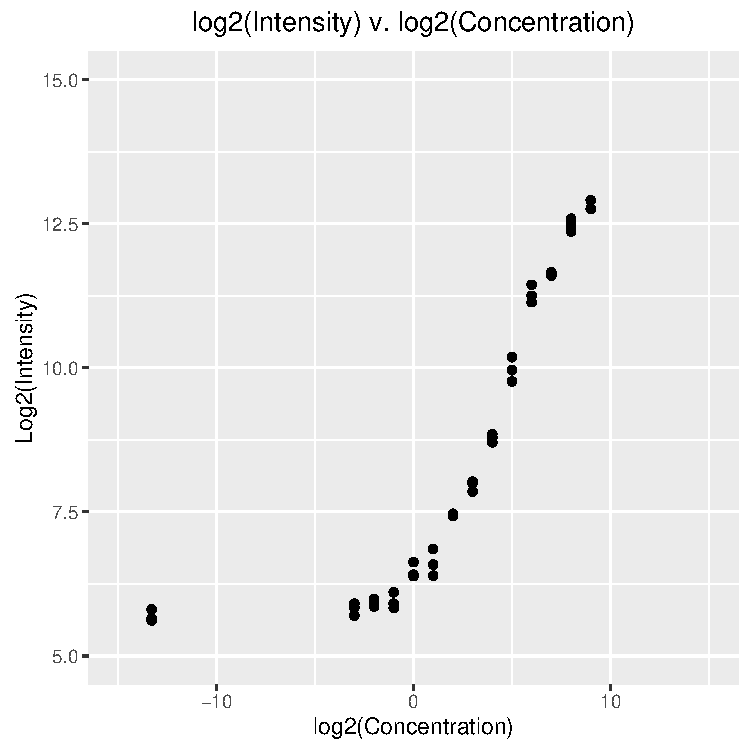
\includegraphics[width=\maxwidth]{figure/chap4-fig1-1} 

\end{knitrout}
\caption{Expression of probe 479376 against concentration on a $\log-\log$ level.}
  \label{fig:c1}
\end{figure}

We can see from looking at this figure that there is a positive relationship (on the $\log$-$\log$ level) between the concentration and expression level of the probe. Notably, however, the relationship is not linear. Indeed the curve tends to flatten out for very high and very low concentrations. One might imagine that the true relationship on this scale is something of a sigmoid curve. We fit such a curve to our data in Figure \ref{fig:c2}.

\begin{figure}[ht]
  \centering
\begin{knitrout}
\definecolor{shadecolor}{rgb}{0.969, 0.969, 0.969}\color{fgcolor}
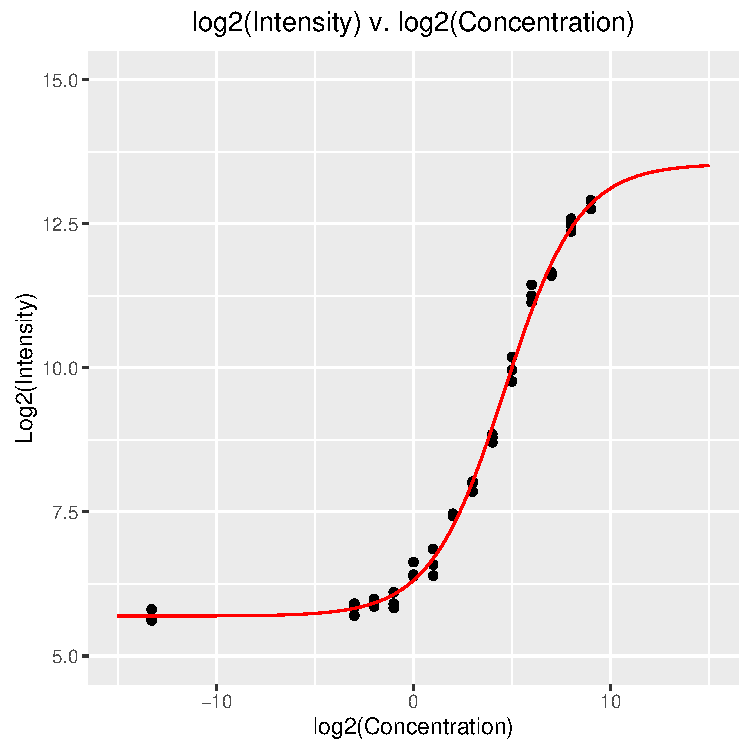
\includegraphics[width=\maxwidth]{figure/chap4-fig2-1} 

\end{knitrout}
\caption{Expression of probe 479376 against concentration on a $\log-\log$ level. Sigmoid curve fit to points.}
  \label{fig:c2}
\end{figure}

This simple sigmoid curve fits the expression-concentration data very well on the $\log$-$\log$ level. The important features of this graph are the flattened tail below about zero, the flattened tail above about eight and, since the sigmoid curve is smooth, the approximately linear relationship between the two tails. In retrospect, this sort of curve isn't too surprising. Indeed some sort of sigmoid curve seems likely given the constraints of the fluorescently activated probes. The probes have a finite maximum amount they can fluorescently shine and hence a saturation point beyond which increasing concentration does not increase expression measurement. This is the right-hand plateau after the $\log_2$ concentration rises above about $8$. On the lower end there is a flat tail on the left-hand side. This is likely because there is some background fluorescence off the microarray probes even when none of the corresponding oligos are present. This might be caused by phenomena like competitive cross hybridization. Thus even as the concentration of the oligo approaches zero the $\log$ intensity doesn't go to negative infinity because there is background fluorescence. Thus we see, instead, the the expression measurement plateau's for low concentrations as well as for high. Both of these phenomena mean that the expression measurement is bounded. Thus the most simple and smooth manner for which the concentration to move from the lower bound to the upper bound as we increase concentration is going to look something like a sigmoid curve. This likely explains why we see such a good fit. Obviously there is no guarantee that there be such a nice relationship between expression and concentration however given the simple continuous fluorescence process it's not too surprising, either.


While this sigmoid curve fits out data quite well we do not use a sigmoidal model in our deconvolution method. Remember that we modeled the $\log_2$ expression, $Y_n$, as linear in the $\log_2$ concentration such that 
\[
Y_n =\log_2(I_n) = \theta_n + \gamma\log_2\left(\eta_n\right) + \epsilon_n
\]
where $\eta_n$ is the concentration of oligo $n$ in the hybridization solution, $\theta_n$ is the oligo-specific intercept, $\gamma$ is the slope for all oligos and $\epsilon_n$ is the oligo-specific error term. We plot such a linear curve for our data in Figure \ref{fig:c3}.

\begin{figure}[ht]
  \centering
\begin{knitrout}
\definecolor{shadecolor}{rgb}{0.969, 0.969, 0.969}\color{fgcolor}
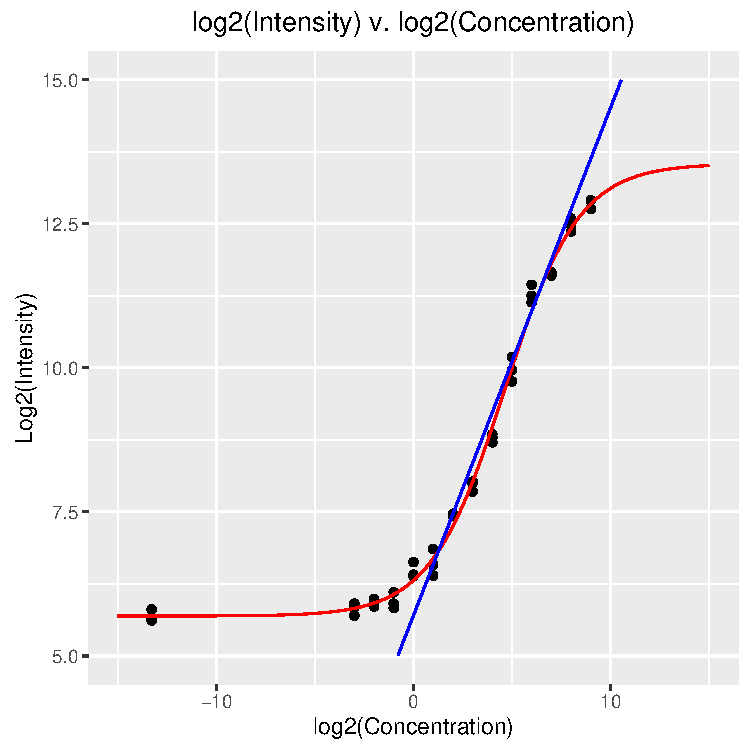
\includegraphics[width=\maxwidth]{figure/chap4-fig3-1} 

\end{knitrout}
\caption{Expression of probe 479376 against concentration on a $\log-\log$ level. Sigmoid fit in red, linear fit in blue.}
  \label{fig:c3}
\end{figure}  

The linear fit in Figure \ref{fig:c3} captures the relationship between the expression and concentration quite well so long as the concentration is not too high nor too low. Obviously the linear fit is not quite as good as the sigmoidal fit however there are some advantages. In the figures plotted in this section we assume we know both concentration and expression. However in a real deconvolution setting we know only the expression and wish to determine the concentration. Indeed our deconvolution method involves using the posited relationship to go from expressions to concentrations. Unfortunately the sigmoidal curve is not a very well behaved curve in this direction. As we increase our expression towards the maximum of our sigmoidal curve the concentration as predicted by the sigmoidal curve will increase without bound. At such high levels of expression small changes in expression will increase the predicted concentration drastically. If instead of working with the red sigmoidal curve we look at the blue linear fit then we see that the predicted concentration does not increase very quickly without bound at such high levels. Indeed it increases linearly with a slope of $\gamma$ at all points. One might view the blue linear fit as some sort of regularized version of the sigmoidal curve which keeps the model from behaving poorly at very high expressions. In a similar sense the linear fit is regularized for low expressions. An expression of, say, five would be predicted as a $\log_2$ concentration near negative infinity from the sigmoidal fit whereas the linear fit predicts a $\log_2$ concentration around zero. Thus our linear fit seems to track the true sigmoidal relationship when the expressions are neither very high nor very small. However for edge cases the linear fit regularizes our estimator keeping the a very highly expressed oligo from dominating the procedure by estimating a very high concentration. At the extreme we see that the red sigmoidal curve has a finite maximum and minimum. Thus if we encounter an expression above or below these extrema our sigmoidal model doesn't give us a straight-forward way of recovering concentration estimates since the curve is not invertible for all real numbers. Our linear model doesn't encounter such problems. For these reasons we choose to model the relationship between concentration and expression in a linear fashion. 
  
\section{A General Model}

Now that we have discussed the manner in which we model the relationship between concentration and expressions let's develop a general model for deconvolution of several cell types by multiple marker oligos. 

Let's assume that we have $K$ cell types under consideration and microarray technology which can measure $N$ oligos. Define $\eta_{kn}$ to be the concentration of oligo $n$ in hybridization solution produced by cells of type $k$ where $k\in\llbracket 1,K\rrbracket$ and $n\in\llbracket 1,N\rrbracket$. Assume that for each cell type $k=1,\ldots,K$ we have $\nu_k$ pure samples of cells of type $k$ only. For each of these samples we generate hybridization solution and run a microarray experiment. From this we get microarray data 
\[
Z_{kr} \in \mathbb{R}^{1\times N}
\]
for $k=1,\ldots,K$ and $r=1,\ldots,\nu_k$. Let's assume that these $Z_{kr}$ are $\log_2$ transformed as previously discussed. In this case then our linear model relating the concentrations $\eta_{kn}$ and the expression measurements $Z_{krn}$ tells us that
\[
Z_{krn} = \theta_n + \gamma \log_2\left(\eta_{kn}\right)+\epsilon_{krn}
\]
where $Z_{krn}$ is the measurement of the $n^{th}$ oligo in the $r^{th}$ pure sample of type $k$ and the $\epsilon_{krn}$ are mutually indpendent across $k,r$ and $n$.

Now assume we also have some heterogeneous sample that is a mixture of the $K$ cell types. This is the sample we would like to deconvolve. Let the hybridization solution of our heterogeneous sample be a mixture of pure sample hybridization solutions with mixing proportions $p_1,\ldots,p_K$. Then if $c_n$ is the concentration of the $n^{th}$ oligo in our heterogeneous sample we have that 
\[
c_n = \sum_{k=1}^{K}p_k\eta_{kn}.
\]

We run DNA microarray analysis on the heterogeneous sample's hybridization solution and get $Y\in\mathbb{R}^{1\times N}$, the $\log_2$ level expressions of oligos $1,\ldots,N$ in the heterogeneous sample. Then our linear model tells us that $Y_n$, the $n^{th}$ oligo expression measurement from this heterogeneous sample, is related to $c_n$ as
\[
Y_n = \theta_n + \gamma\log_2\left(c_n\right)+\epsilon_n.
\]
We assume that the $\epsilon_n$ and the $\epsilon_{krn}$ from the pure samples are mutually independent with mean zero and some finite fixed variance $\sigma^2$.

In order to deconvolve the heterogeneous sample assume there are some number of marker oligos for each cell type $k\in\llbracket1, K\rrbracket$. Let $G_k\subset\llbracket 1, N\rrbracket$ be the set of marker oligos for cell type $k$ such that if $n \in G_k$ then $\eta_{tn}=0$ for all $t \neq k$. That is, if $n$ is a marker oligo of cell type $k$ then it is not expressed in any other cell type than $k$. Assume that the marker oligos are mutually exclusive across cell types such that $G_k\cap G_t=\emptyset$ for all $t \neq k$. 

Now consider some oligo $n$ that is a marker of cell type $k$ such that $n\in G_k$. Then we have that
\[
c_n = \sum_{t=1}^{K} \eta_{tn}p_t = \eta_{kn} p_k
\]
as $\eta_{tn}=0$ for all $t\neq k$.
That is, if $n$ is a marker oligo of cell type $k$ then the concentration of $n$ in the heterogeneous sample is simply the concentration of $n$ in any of the pure type-$k$ samples, $\eta_{kn}$, scaled down by the mixing proportion $p_k$.

Thus if $n\in G_k$ we have that 
\[
\begin{aligned}
  Y_n &=\theta_n + \gamma\log_2\left(c_n\right)+\epsilon_n\\
  &= \theta_n + \gamma\log_2\left(\eta_{nk}p_k\right)+\epsilon_n\\
  &= \theta_n + \gamma\log_2\left(\eta_{nk}\right)+\gamma\log_2\left(p_k\right)+\epsilon_n 
\end{aligned}
\]
and
\[
\begin{aligned}
  \overline{Z_{kn}}\overset{def}{=}\frac{1}{\nu_k}\sum_{r=1}^{\nu_k}Z_{krn} &= \frac{1}{\nu_k}\sum_{r=1}^{\nu_k}\left(\theta_n + \gamma \log_2\left(\eta_{kn}\right)+\epsilon_{krn}\right)\\
  &= \theta_n + \gamma \log_2\left(\eta_{kn}\right)+\overline{\epsilon_{kn}}
\end{aligned}
\]
where $\overline{\epsilon_{kn}} \overset{def}{=} \frac{1}{\nu_k}\sum_{r=1}^{\nu_k}\epsilon_{krn}$. Thus
\[
  Y_n - \overline{Z_{kn}} = \gamma\log_2\left(p_k\right)+\epsilon_n - \overline{\epsilon_{kn}}
\]
and so if we average such terms over all marker oligos $n\in G_k$ we get
\[
\begin{aligned}
E_k &\overset{def}{=} \frac{1}{\Gamma_k} \sum_{n\in G_k}\left(Y_n-\overline{Z_{kn}}\right)\\
&=\frac{1}{\Gamma_k} \sum_{n\in G_k} \left(\gamma\log_2\left(p_k\right)+\epsilon_n - \overline{\epsilon_{kn}}\right)\\
&=\gamma\log_2\left(p_k\right)+\frac{1}{\Gamma_k} \sum_{n\in G_k}\left(\epsilon_n - \overline{\epsilon_{kn}}\right)
\end{aligned}
\]
where $\Gamma_k \overset{def}{=} |G_k|$. If we knew $\gamma$ then we could solve for $p_k$, approximately, as
\[
\exp_2\left(\frac{E_k}{\gamma}\right) = \lambda_k p_k
\]
where $\lambda_k = \exp_2\left(\frac{1}{\Gamma_k} \sum_{n\in G_k}\left(\epsilon_n - \overline{\epsilon_{kn}}\right)\right)$ is some multiplicative error term. Since we don't know $\gamma$ let's suppose we can estimate $\gamma$ by some estimator $\widehat{\gamma}$ and then plug into the previous equation to get an estimator 
\[
\widehat{q_k} = \exp_2\left(\frac{E_k}{\widehat{\gamma}}\right)
\]
with the hopes that if $\widehat{\gamma}\rightarrow\gamma$ then $\widehat{q_k}\rightarrow \lambda_kp_k$.

Ideally these $\widehat{q_k}$ would be our final estimators of the $p_k$. However in reality there is no guarantee that the collection of these $\widehat{q_k}$ are bounded above by one and sum to one. So we opt instead to re-normalize the $\widehat{q_k}$ and define the estimators
\[
\widehat{p_k} = \frac{\widehat{q_k}}{\sum_{t=1}^{K}\widehat{q_t}}
\]
as our final estimators of the $p_k$. These $\widehat{p_k}$ are all non-negative and sum to one as desired. 

In the next section we will contrast our estimators with those discussed in the literature. Then we will dig into the details of how to estimate $\gamma$ and how to choose the marker oligos.

\section{Comparison}

Let's compare our method to the most similar methods existing in the deconvolution literature. Our method estimated the mixing proportions $p_k$ through relationships between the $p_k$, $Y$, and the $Z_{kr}$ where $Y$ and $Z_{kr}$ are $\log$-level expression measurements. Some of the methods in the literature worked at the linear level working instead with $X$ and $W_{kr}$ such that $Y_n = \log_2(X_n)$ and $Z_{krn}=\log_2(W_{krn})$ so that $X$ and the $W_{krn}$ are the linear-level expression measurements. These methods would use the microarray expressions from pure samples, the $W_{kr}$, to choose marker genes and generate pure cell type expression profiles as encoded in the profile matrix $U\in\mathbb{R}^{K\times N}$. One obvious way to create $U$ is to let the $k^{th}$ row of $U$ be the average of $W_{kr}$ from $r=1,\ldots,\nu_k$. That is,
\[
U_k = \frac{1}{\nu_k} \sum_{r=1}^{\nu_k}W_{kr}
\]
so that $U$ is the matrix of characteristic expression profiles of the $K$ types in so much as row $k$ is the typical expressions of the $N$ oligos in a pure sample of cell type $k$. 
From here the model assumes that $M=(p_1,\ldots,p_K) \in \mathbb{R}^{1\times K}$ and posits the relationship
\[
X = MU + E
\]
where $E\in\mathbb{R}^{1\times N}$ is some random matrix of errors. Thus, 
\[
X_n = \sum_{k=1}^{K}p_kU_{kn}+e_{n}
\]
so that the model posits that for each oligo $n$ the expression measurement in the heterogeneous sample, $X_n$, is a convex combination of the expression of this oligo in each of the pure samples (i.e. the characteristic profiles) $U_{kn}$ with weights as the mixing proportions $p_k$ and some error term $e_n$. If we $\log$-transform both sides then we get that the model posits
\begin{equation}
\label{eqn:complit}
Y_n = \log_2\left(X_n\right) = \log_2\left(\sum_{k=1}^{K}p_kU_{kn}+e_{n}\right).
\end{equation}
Compare this to the linear model our method posits. We model the relationships as 
\[
c_n = \sum_{k=1}^{K}p_k\eta_{kn}
\]
and 
\[
Y_n = \theta_n + \gamma\log_2\left(c_n\right)+\epsilon_n
\]
so that
\begin{equation}
\label{eqn:compours}
Y_n = \theta_n + \gamma\log_2\left(\sum_{k=1}^{K}p_k\eta_{kn}\right)+\epsilon_n.
\end{equation}

There are striking simliarities between a standard model posited in the literature in Equation \ref{eqn:complit} and our model in Equation \ref{eqn:compours}. Both equations model the $Y_n$ as the $\log$ of a convex combination with weights that are the mixing proportions $p_1,\ldots,p_K$. However there are several important differences between the methods. First is the placement of the error terms $e_n$ and $\epsilon_n$. Secondly, there are differences in the terms in the convex combination. Thirdly, our model includes slope and intercept terms $\gamma$ and $\theta_n$. Finally, although not aparent from the modeling equations alone, there are differences in fitting methods among the models. 

The differenes in the placements of the error terms is not very important. This essentially arises because one model is fit at the linear level and the other is fit on the $\log$ level. More importantly, most of the methods in literature do ont explicitly include a random error term. We add an error term to their models assuming that since they estimate the $p_k$ by by minimizing terms like $||X-MU||$ over $M$ they are implicitly assuming some sort of linear error term at the linear level. The authors put very little emphasis on such terms and hence focusing on something the authors do not explicitly state does not seem important. 

The second difference between our model and a typical model in the literature is that while our model posits $Y_n$ is dependent on the $\log$ of the convex combination $\sum_{k=1}^{K}p_k\eta_{kn}$ those models in the literature instead assume that $Y_n$ is dependent on the log of the convex combination $\sum_{k=1}^{K}p_kU_{kn}$. The difference here being that the models in the literature assume some sort of direct relationship of $Y_n$ on the characteristic \emph{expressions} $U_{kn}$ while our model posits a relationship of $Y_n$ on the \emph{concentrations} of such oligos in the pure sampes, $\eta_{kn}$. Thus our model uses concentrations while theirs use expressions.  Now obviously the characteristic expression profiles $U_{kn}$ are typical generated from such pure sample expressions $W_{krn}$ and thus themselves depend on the concentration of the oligos $\eta_{kn}$. However the oligo expressions $W_{krn}$ and the oligo concentrations $\eta_{kn}$ are not interchagable. Most methods in the literature seem to assume that they are. That is, most methods to date assume that the expression measurements from the microarrays are indistinguishable from the concentration of those oligos in the samples. The implicit assumption is that the expressions directly give us the concentration of the oligos. Obviously there is a relationship between the expressions and the concentrations. However in our method we separate the two quantites modeling the expressions as a linear function of the concentrations. We believe that this distinction is crucial to accurate modeling of the convolution phenomena. Effectively most methods in the literature assume that $W_{krn} = \eta_{krn}$ such that $Z_{krn} = \log_2\left(\eta_{kn}\right)$ while in our method we model the relationship as $Z_{krn}=\theta_n+\gamma\log_2\left(\eta_{kn}\right)+\epsilon_{krn}$ including an intercept $\theta_n$ and a slope $\gamma$ to explain the relationship. This difference in modeling can be seen again in the modeling equation of $Y_n$. In Equation \ref{eqn:compours} we include the slope and intercept when modeling the dependence of $Y_n$ on $\log_2\left(\sum_{k=1}^{K}p_k\eta_{kn}\right)$ while the prototypical method in the literature typified by Equation \ref{eqn:complit} directly set $Y_n$ equal to $\log_2\left(\sum_{k=1}^{K}p_kU_{kn}\right)$. Thus our model is more complex than those in the literature because it introduces intercept parameters $\theta_n$ and a slope parameter $\gamma$. Notice that if we set each of these $\theta_n$ to zero and $\gamma$ to be one then we get something very similar to Equation \ref{eqn:complit}.

While there are some similarities in the models used by methods in the existing literature and those used in our method there are big differences in how the two models are fit. Most of the methods in the literature view the $p_k$ as parameters in a linear model and estimate the $p_k$ according to some classic method like least squares or convex optimization. For our technique we do not view the mixing proportions as parameters in a linear model. Instead we estimate our slope parameter $\gamma$ from an independent data set and then solve for the mixing proportions directly in the model using information from the pure samples to account for the $\theta_n$ and the $\eta_{kn}$. The fitting method is much different than any of the classic methods used in the literature. Furthermore our method distinguishes itself from other algorithms by the data on which it works. Most other methods work on data that has been highly pre-processed by algorithms like RMA or MAS5. Those algorithms summarize the low-level probe data into gene-level data. While looking at gene-level data in this way can be helpful our method does not require any such preprocessing. Instead we work with very low level raw intensity measurements from the microarrays at the level of probes on the array rather than summarizations of probes into genes. 

Finally it should be noted that the conversation in this section was based upon algorithms that modeled the expressions as linear at the linear (non-$\log$) level. The models used such  linear-level algorithms are most comparable to our own. Thus our conversation has focused upon them. However fully half of the algorithms we reviewed in the literature were not such models. Indeed many methods modeled expressions as linear relationships at the $\log$ level. These types of algorithms are even more different to our own. Briefly, $\log$-level models typical model the expression as something along the lines of 
\[
Y_n = \sum_{k=1}^{K}p_k \log_2\left(U_{kn}\right) + e_{n}
\]
which is a completely different model than ours. Adding an intercept $\theta_n$ and slope $\gamma$ will not reconcile the differences between these $\log$-based models and ours since the summation and parameters $p_k$ have been brought outside the $\log$.

In conclusion then there are some methods which model expressions as linear models at the linear level. These are similar to our algorithm however they use a much simpler model than our own. There are also methods which model expressions as linear at the $\log$ level. These models are fundamentally different than the model we propose. In any case, algorithms at both the linear and $\log$ levels fit their parameters as classic linear models which is much different to our estimation procedure. 


\section{Estimating $\gamma$ and Choosing Markers.}

The estimators $\widehat{p_k}$ depend on being able to estimate $\gamma$ and being able to choose marker oligos for each of the types. Here we will discuss the details of how those tasks are accomplished. 
  
\subsection{Estimating $\gamma$}
  
Now the parameter $\gamma$ is a global parameter which does not depend on which oligo measurement we are considering. Indeed if the precise pre-processing of our data $Y$ is fixed then this parameter can be estimated once for all data sets. The ability to do such an estimation depends on the existence of a data set linking the concentration (or amounts) of oligos in a data set with the expression measurements by the profiling technology. 

For technology like DNA microarrays there are many such data sets from which we can estimate $\gamma$. In particular we use the Latin Square data set (\cite{latin}). In this experiment a DNA microarray was performed on several samples in which were spiked in a common background human RNA cocktail as well as particular oligonucleotides at known concentrations. A simple linear regression model was then fit to trimmed data regressing expression levels on concentration for those measurements with known concentration. The estimated slope from this model was then used as $\widehat{\gamma}$. This method is very simple and can definitely be improved. It also requires that there be data sets with known concentrations and expressions. Nicely, however, $\gamma$ needs only be estimated once for each technology and normalization regime. 

\subsection{Choosing Markers}

The last step in describing our complete deconvolution algorithm is to describe the manner in which marker oligos are chosen. As discussed in Chapter \ref{chap:Lit} there is quite a bit of variety in how marker genes are chosen. Here we decide to leverage the DNA microarray experiments on pure samples, those $Z_{kr}$, to determine which oligos are indicative of one, and only one, type. To do this let 
$$
Z_n = ((Z_{11})_n,\ldots,(Z_{1R_1})_n,(Z_{21})_n,\ldots,(Z_{2R_2})_n,\ldots,(Z_{K1})_n,\ldots (Z_{KR_K})_n)
$$
be the measurements of the $n^{th}$ oligo across all the $Z_{kr}$. Similarly let $X_k$ be the indicator for $Z$ such that $(X_k)_i=1$ if and only if $(Z_n)_i$ is a measurement coming from a pure cell sample of type $k$. Precisely, we say that if $R_{k^-} = \sum_{i=1}^{k-1} R_i$ then $(X_K)_i = 1$ if $R_{k^-} < i \leq R_{{(k+1)}^{-}}$ and zero elsewhere. For each $n$ and $k$ we fit the simple linear regression of $Z_n$ on $X_k$ and estimate a slope $\widehat{\beta_{kn}}$. Using these slopes we assign a top type to each oligo $n$ defining sets $\tau_k$ of the top oligos for each cell type $k$ so that 
$$
\tau_k = \left\{n \left| k=\arg\max_{t=1,\ldots,K}\widehat{\beta_{tn}}\right.\right\}
$$
so that $\tau_k\subset \llbracket 1,n \rrbracket$ is the set of oligos for which cell type $k$ has the largest slope among the regressions. 
Given some parameter $M$, the number of marker oligos we wish to use, we then define the marker oligos for type $k$ as
$$
G_k = \left\{n \in \tau_k \left|\widehat{\beta_{kn}} \geq \widehat{\beta_{k(M)}}\right.\right\}
$$
where $\widehat{\beta_{k(M)}}$ is the $M^{th}$ order statistic of the set $\left\{\widehat{\beta_{kn}}\left|n\in\tau_k\right.\right\}$. This is to say that $G_k$, the set of marker oligos for cell type $k$, is comprised of the set of oligos $n$ for which the slope $\widehat{\beta_{kn}}$ is one of the top $M$ slopes among all oligos where cell type $k$ has the largest slope across all cell types. 

The slopes from our regression of $Z_n$ on the indicator $X_k$ tell us about how much the oligo $n$ differentiates cell type $k$ from all other oligos. Thus we pick those oligos to be markers if they are the best at discriminating between cell type $k$ and the other types. Implicit in having a large regression slope is that the oligo $n$ must be much more expressed in cell type $k$ than other types. Thus satisfying the definition of a marker oligo. There are definitely simpler ways of choosing marker oligos which give good results. However our hope is to extend and robustify this marker oligo selection using methods like RUV \citet{Gagnon-Bartsch2012}. In this light, then, the regression framework is useful. Choosing the marker oligos is a very important step in any deconvolution algorithm thus much of our future work will focus on exploring precisely how to do this well. This includes determining how many marker oligos, $M$, to pick for each cell type. 

 \chapter{Analysis on Real Data}
 \label{chap:Analysis}


\section{Methods and Implementations}

our method 
-- say it's available on github
-- basically just choose 1000 marker

their methods
-- mention methods and citations
-- say cell mix
-- say how genes are chosen
-- say linear level
-- appendix for code

\section{The Rat Data Set}

\begin{figure}
  \centering
\begin{knitrout}
\definecolor{shadecolor}{rgb}{0.969, 0.969, 0.969}\color{fgcolor}
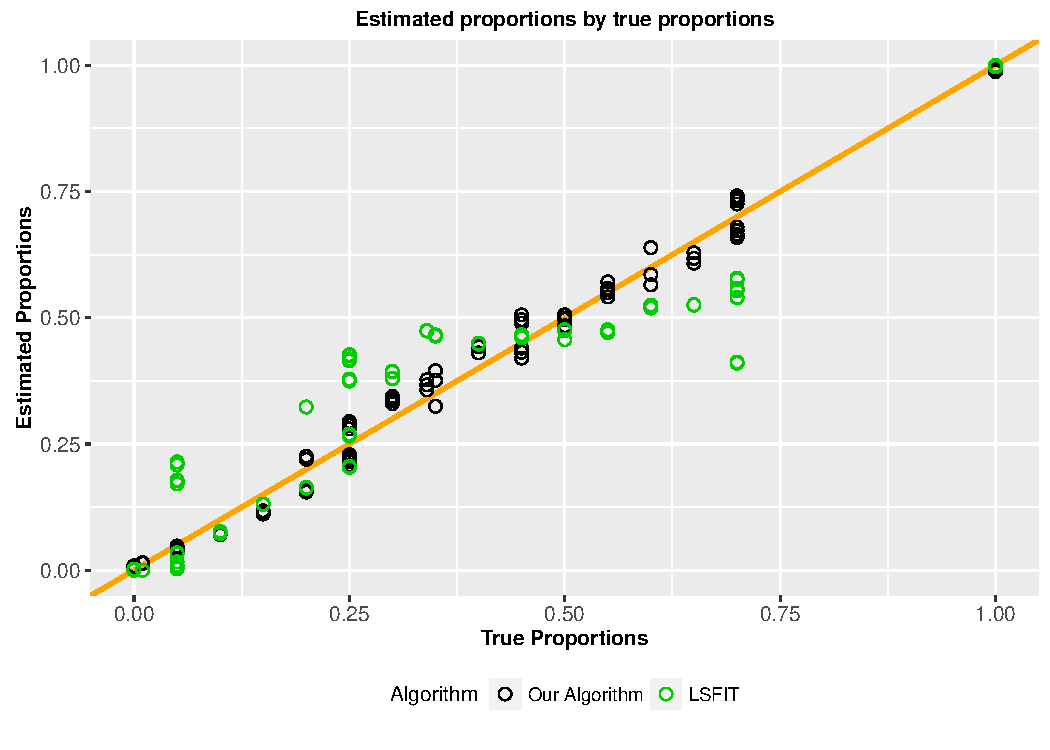
\includegraphics[width=\maxwidth]{figure/plot1-1} 

\end{knitrout}
\end{figure}

\begin{figure}
  \centering
\begin{knitrout}
\definecolor{shadecolor}{rgb}{0.969, 0.969, 0.969}\color{fgcolor}
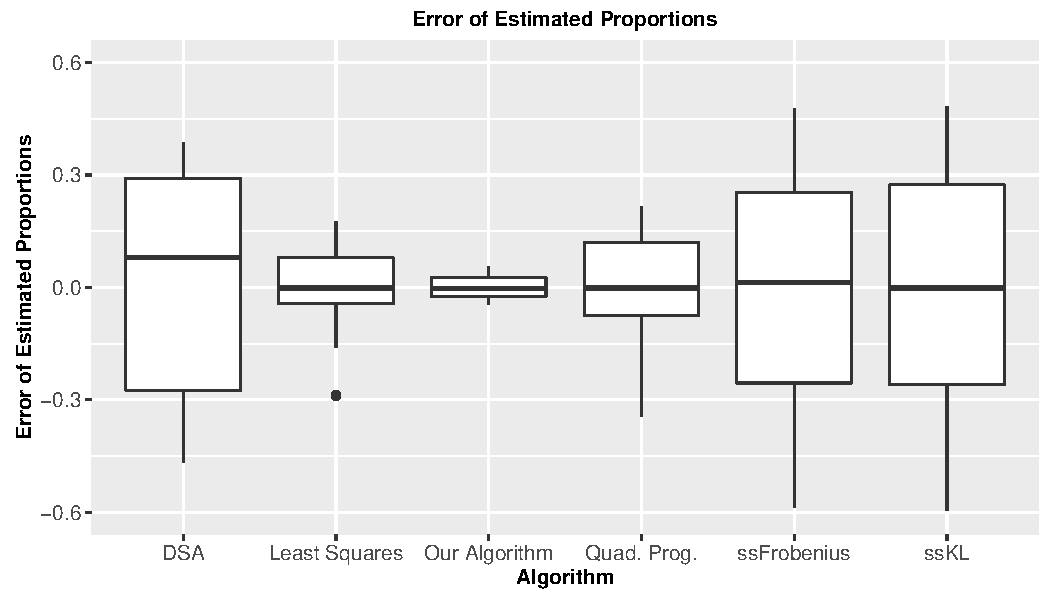
\includegraphics[width=\maxwidth]{figure/plot2-1} 

\end{knitrout}
\end{figure}

% latex table generated in R 3.3.1 by xtable 1.8-2 package
% Wed Nov 23 17:21:06 2016
\begin{table}[ht]
\centering
\begin{tabular}{lllllll}
  \hline
Percentile & Our Algorithm & DSA & Least Squares & Quad. Prog. & ssKL & ssFrobenius \\ 
  \hline
0\% & 0 & 0.003 & 0 & 0 & 0.002 & 0.004 \\ 
  25\% & 0.009 & 0.102 & 0.017 & 0.022 & 0.11 & 0.109 \\ 
  50\% & 0.025 & 0.28 & 0.046 & 0.1 & 0.269 & 0.255 \\ 
  75\% & 0.036 & 0.358 & 0.124 & 0.162 & 0.346 & 0.341 \\ 
  100\% & 0.056 & 0.76 & 0.29 & 0.344 & 0.655 & 0.667 \\ 
   \hline
\end{tabular}
\end{table}


\section{The Blood Data set}

\begin{figure}
  \centering
\begin{knitrout}
\definecolor{shadecolor}{rgb}{0.969, 0.969, 0.969}\color{fgcolor}
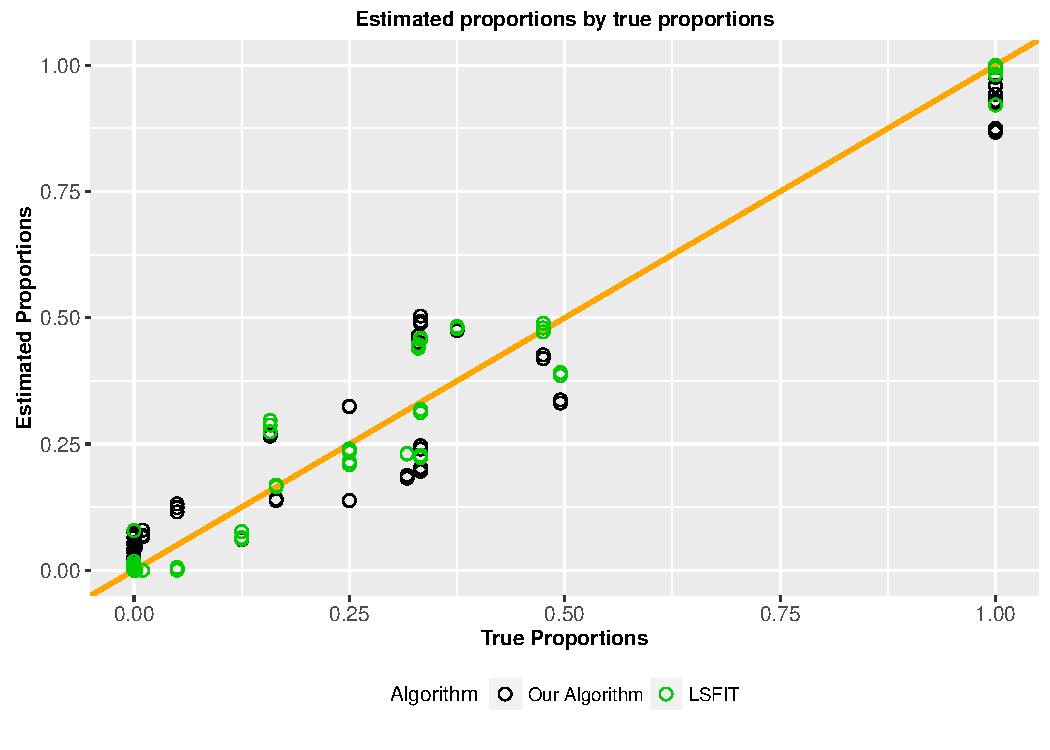
\includegraphics[width=\maxwidth]{figure/plot3-1} 

\end{knitrout}
\end{figure}

\begin{figure}
  \centering
\begin{knitrout}
\definecolor{shadecolor}{rgb}{0.969, 0.969, 0.969}\color{fgcolor}
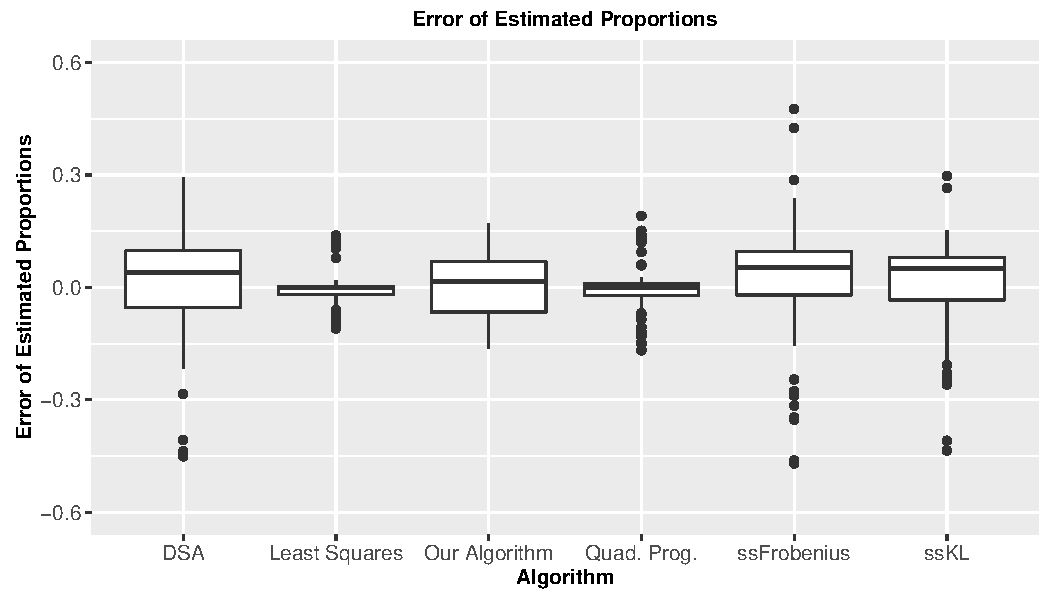
\includegraphics[width=\maxwidth]{figure/plot4-1} 

\end{knitrout}
\end{figure}

% latex table generated in R 3.3.1 by xtable 1.8-2 package
% Wed Nov 23 17:21:07 2016
\begin{table}[ht]
\centering
\begin{tabular}{lllllll}
  \hline
Percentile & Our Algorithm & DSA & Least Squares & Quad. Prog. & ssKL & ssFrobenius \\ 
  \hline
0\% & 0.006 & 0.001 & 0 & 0 & 0.02 & 0 \\ 
  25\% & 0.034 & 0.046 & 0.001 & 0.001 & 0.049 & 0.052 \\ 
  50\% & 0.068 & 0.077 & 0.013 & 0.015 & 0.076 & 0.076 \\ 
  75\% & 0.112 & 0.123 & 0.086 & 0.109 & 0.137 & 0.187 \\ 
  100\% & 0.171 & 0.451 & 0.139 & 0.191 & 0.435 & 0.789 \\ 
   \hline
\end{tabular}
\end{table}




 
 \chapter{Conclusion}
 \label{chap:Conclusion}


\lipsum[2]

\section{Future Work}

\lipsum[3]
 

\renewcommand{\bibsection}{}
\startbibliography
 \begin{singlespace} % Bibliography must be single spaced
  \bibliography{Deconvolution,other}
 \end{singlespace}
 
\startappendices
\appendix{Code Appendix}

\begin{center}
Chapter \ref{chap:Method} Knitr Code (\href{https://github.com/gjhunt/prelim/blob/master/Method.R}{Method.R})
\end{center}
\input{append_code/Method.Rsource}

\begin{center}
  Chapter \ref{chap:Method} Figure 1 (\href{https://github.com/gjhunt/prelim/blob/master/Method/latin_R/chap4-fig1.R}{Method/latin\_R/chap4-fig1.R})
\end{center}
\input{append_code/chap4-fig1.Rsource}

\begin{center}
 Chapter \ref{chap:Method} Figure 2 (\href{https://github.com/gjhunt/prelim/blob/master/Method/latin_R/chap4-fig2.R}{Method/latin\_R/chap4-fig2.R})
 \end{center}
\input{append_code/chap4-fig2.Rsource}

 \lstinputlisting[language=R,caption={Chapter \ref{chap:Method} Figure 3 (\href{https://github.com/gjhunt/prelim/blob/master/Method/latin_R/chap4-fig3.R}{Method/latin\_R/chap4-fig3.R})}]{Method/latin_R/chap4-fig3.R}
  \lstinputlisting[language=R,caption={Chapter \ref{chap:Method} Latin Square Preprocessing (\href{https://github.com/gjhunt/prelim/blob/master/Method/latin_R/latin_data_read.R}{Method/latin\_R/latin\_data\_read.R})}]{Method/latin_R/latin_data_read.R}
  \lstinputlisting[language=R,caption={Chapter \ref{chap:Method} Latin Square Fitting Routine (\href{https://github.com/gjhunt/prelim/blob/master/Method/latin_R/latin_data_plot.R}{Method/latin\_R/latin\_data\_plot.R})}]{Method/latin_R/latin_data_plot.R}

    
 \lstinputlisting[language=R,caption={Chapter \ref{chap:Analysis} Knitr Code (\href{https://github.com/gjhunt/prelim/blob/master/Analysis.R}{Analysis.R})}]{Analysis.R}
 \lstinputlisting[language=R,caption={Chapter \ref{chap:Analysis} Analysis script (\href{https://github.com/gjhunt/prelim/blob/master/Analysis/R/Analysis_script.R}{Analysis/R/Analysis\_script.R})}]{Analysis/R/Analysis_script.R}
\lstinputlisting[language=R,caption={Chapter \ref{chap:Analysis} Data Reading Script (\href{https://github.com/gjhunt/prelim/blob/master/Analysis/R/read_data.R}{Analysis/R/read\_data.R})}]{Analysis/R/read_data.R}
 \lstinputlisting[language=R,caption={Chapter \ref{chap:Analysis} Helper Script (\href{https://github.com/gjhunt/prelim/blob/master/Analysis/R/update.R}{Analysis/R/update.R})}]{Analysis/R/update.R}



% An external Abstract that can be printed at the end of the document, 
% for separate submission to Rackham. Comment it out when not needed. - jg
%\startextabstractpage
%{The Title of Your Dissertation}{Your Name}{Chair: Albert Einstein}
%\input{Abstract/Abstract}
%\label{ExtAbstract}

\end{document}
